\begin{enumerate}[label=\thesection.\arabic*,ref=\thesection.\theenumi]
\numberwithin{equation}{enumi}
\numberwithin{figure}{enumi}
\numberwithin{table}{enumi}

    \item Draw a quadrilateral in the Cartesian plane, whose vertices are 
    \begin{align}
        \vec{A} = \myvec{-4\\5} \quad \vec{B} = \myvec{0\\7} \\
        \vec{C} = \myvec{5\\-5} \quad \vec{D} = \myvec{-4\\-2}
    \end{align}
    Also, find its area.
\label{chapters/11/10/1/1}
   \\ 
    \solution 
\iffalse
\documentclass[journal,12pt,twocolumn]{IEEEtran}
\usepackage{setspace}
\usepackage{gensymb}
\usepackage{xcolor}
\usepackage{caption}
\singlespacing
\usepackage{siunitx}
\usepackage[cmex10]{amsmath}
\usepackage{mathtools}
\usepackage{hyperref}
\usepackage{amsthm}
\usepackage{mathrsfs}
\usepackage{txfonts}
\usepackage{stfloats}
\usepackage{cite}
\usepackage{cases}
\usepackage{subfig}
\usepackage{longtable}
\usepackage{multirow}
\usepackage{enumitem}
\usepackage{mathtools}
\usepackage{listings}
\usepackage{tikz}
\usetikzlibrary{shapes,arrows,positioning}
\usepackage{circuitikz}
\let\vec\mathbf
\DeclareMathOperator*{\Res}{Res}
\renewcommand\thesection{\arabic{section}}
\renewcommand\thesubsection{\thesection.\arabic{subsection}}
\renewcommand\thesubsubsection{\thesubsection.\arabic{subsubsection}}

\renewcommand\thesectiondis{\arabic{section}}
\renewcommand\thesubsectiondis{\thesectiondis.\arabic{subsection}}
\renewcommand\thesubsubsectiondis{\thesubsectiondis.\arabic{subsubsection}}
\hyphenation{op-tical net-works semi-conduc-tor}

\lstset{
language=Python,
frame=single, 
breaklines=true,
columns=fullflexible
}
\begin{document}
\theoremstyle{definition}
\newtheorem{theorem}{Theorem}[section]
\newtheorem{problem}{Problem}
\newtheorem{proposition}{Proposition}[section]
\newtheorem{lemma}{Lemma}[section]
\newtheorem{corollary}[theorem]{Corollary}
\newtheorem{example}{Example}[section]
\newtheorem{definition}{Definition}[section]
\newcommand{\BEQA}{\begin{eqnarray}}
\newcommand{\EEQA}{\end{eqnarray}}
\newcommand{\define}{\stackrel{\triangle}{=}}
\newcommand{\myvec}[1]{\ensuremath{\begin{pmatrix}#1\end{pmatrix}}}
\newcommand{\mydet}[1]{\ensuremath{\begin{vmatrix}#1\end{vmatrix}}}

\bibliographystyle{IEEEtran}
\providecommand{\nCr}[2]{\,^{#1}C_{#2}} % nCr
\providecommand{\nPr}[2]{\,^{#1}P_{#2}} % nPr
\providecommand{\mbf}{\mathbf}
\providecommand{\pr}[1]{\ensuremath{\Pr\left(#1\right)}}
\providecommand{\qfunc}[1]{\ensuremath{Q\left(#1\right)}}
\providecommand{\sbrak}[1]{\ensuremath{{}\left[#1\right]}}
\providecommand{\lsbrak}[1]{\ensuremath{{}\left[#1\right.}}
\providecommand{\rsbrak}[1]{\ensuremath{{}\left.#1\right]}}
\providecommand{\brak}[1]{\ensuremath{\left(#1\right)}}
\providecommand{\lbrak}[1]{\ensuremath{\left(#1\right.}}
\providecommand{\rbrak}[1]{\ensuremath{\left.#1\right)}}
\providecommand{\cbrak}[1]{\ensuremath{\left\{#1\right\}}}
\providecommand{\lcbrak}[1]{\ensuremath{\left\{#1\right.}}
\providecommand{\rcbrak}[1]{\ensuremath{\left.#1\right\}}}
\theoremstyle{remark}
\newtheorem{rem}{Remark}
\newcommand{\sgn}{\mathop{\mathrm{sgn}}}
\newcommand{\rect}{\mathop{\mathrm{rect}}}
\newcommand{\sinc}{\mathop{\mathrm{sinc}}}
\providecommand{\abs}[1]{\left\vert#1\right\vert}
\providecommand{\res}[1]{\Res\displaylimits_{#1}} 
\providecommand{\norm}[1]{\left\Vert#1\right\Vert}
\providecommand{\mtx}[1]{\mathbf{#1}}
\providecommand{\mean}[1]{E\left[ #1 \right]}
\providecommand{\fourier}{\overset{\mathcal{F}}{ \rightleftharpoons}}
\providecommand{\ztrans}{\overset{\mathcal{Z}}{ \rightleftharpoons}}
\providecommand{\system}[1]{\overset{\mathcal{#1}}{ \longleftrightarrow}}
\newcommand{\solution}{\noindent \textbf{Solution: }}
\providecommand{\dec}[2]{\ensuremath{\overset{#1}{\underset{#2}{\gtrless}}}}
\let\StandardTheFigure\thefigure
\def\putbox#1#2#3{\makebox[0in][l]{\makebox[#1][l]{}\raisebox{\baselineskip}[0in][0in]{\raisebox{#2}[0in][0in]{#3}}}}
     \def\rightbox#1{\makebox[0in][r]{#1}}
     \def\centbox#1{\makebox[0in]{#1}}
     \def\topbox#1{\raisebox{-\baselineskip}[0in][0in]{#1}}
     \def\midbox#1{\raisebox{-0.5\baselineskip}[0in][0in]{#1}}

\vspace{3cm}
\title{Straight Lines Assignment}
\author{Gautam Singh}
\maketitle
\bigskip

\begin{abstract}
    This document contains the solution to Question 1 of Exercise 1 in Chapter
    10 of the class 11 NCERT textbook.
\end{abstract}

\begin{enumerate}
\fi
		The points are plotted in Fig. \ref{fig:11/10/1/1quad}. The plot is 
    generated using the Python code \texttt{codes/quad.py}.

    The area vector (denoted by $\vec{R_X}$ for region $X$) of the quadrilateral 
    is perpendicular to the plane of the quadrilateral and its orientation is 
    assumed to be in the positive $z$-direction here.
    \begin{align}
        &\vec{R_{ABCD}} = \vec{R_{ABC}} + \vec{R_{ACD}} \\
        &= \frac{1}{2}\brak{\brak{\vec{B}-\vec{A}}\times\brak{\vec{C}-\vec{A}} + 
        \brak{\vec{C}-\vec{A}}\times\brak{\vec{D}-\vec{A}}} \\
        &= \frac{1}{2}\brak{\brak{\vec{C}-\vec{A}}\times
        \brak{\vec{D}-\vec{A}+\vec{A}-\vec{B}}} \\
        &= \frac{1}{2}\brak{\brak{\vec{C}-\vec{A}}\times\brak{\vec{D}-\vec{B}}} \\
        \label{eq:11/10/1/1area-diag} 
    \end{align}
    Thus the area of quadrilateral ABCD is
    \begin{align}
        \textrm{ar}\brak{ABCD} &= \norm{\vec{R_{ABCD}}} \\
                               &= \frac{1}{2}\norm{\brak{\vec{C}-\vec{A}}\times\brak{\vec{D}-\vec{B}}} \\ 
                               &= \frac{1}{2}\mydet{9&-4\\-10&-9} \\
                               &= 60.5\ \textrm{sq. units.}
        \label{eq:11/10/1/1ans}
    \end{align}
    \begin{figure}[!htb]
        \centering
        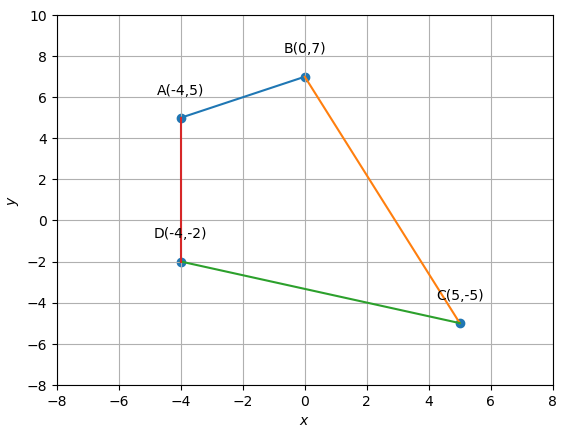
\includegraphics[width=\columnwidth]{chapters/11/10/1/1/figs/quad.png}
        \caption{Plot of quadrilateral $ABCD$}
        \label{fig:11/10/1/1quad}
    \end{figure}

\item 
\label{chapters/11/10/1/2}
\iffalse
\documentclass[journal,12pt,twocolumn]{IEEEtran}
\usepackage{graphicx}
\usepackage{listings}
\usepackage[utf8]{inputenc}
\usepackage{caption}
\usepackage{hyperref}
\usepackage[cmex10]{amsmath}
\usepackage{array}
\usepackage{gensymb}
\usepackage{booktabs}
\usepackage{etoolbox}
\patchcmd{\section}{\centering}{}{}{}
\providecommand{\norm}[1]{\left\lVert#1\right\rVert}
\providecommand{\abs}[1]{\left\vert#1\right\vert}
\let\vec\mathbf
\newcommand{\myvec}[1]{\ensuremath{\begin{pmatrix}#1\end{pmatrix}}}
\newcommand{\mydet}[1]{\ensuremath{\begin{vmatrix}#1\end{vmatrix}}}
\providecommand{\brak}[1]{\ensuremath{\left(#1\right)}}
\makeatletter
\newcommand\xleftrightarrow[2][]{%
  \ext@arrow 9999{\longleftrightarrowfill@}{#1}{#2}}
\newcommand\longleftrightarrowfill@{%
  \arrowfill@\leftarrow\relbar\rightarrow}
\makeatother
\title{Matrix Problems \textbf{\\Straight Lines }}
\author{Manoj Chavva} 

\begin{document}
\maketitle



\section{Problem Statement}

\noindent 
\fi
The base of an equilateral triangle with side $2a$ lies along the y-axis such that the mid-point of the base is at the origin. Find vertices of the triangle.
	\begin{figure}[!ht]
		\centering
 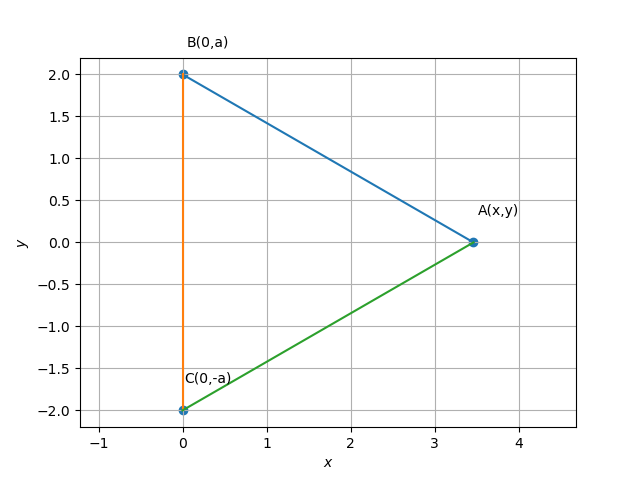
\includegraphics[width=\columnwidth]{chapters/11/10/1/2/figs/triangle.png}
		\caption{}
		\label{fig:11/10/1/2}
  	\end{figure}
	\\
	\solution Let the base be $BC$.  From the given information, 
\begin{align}
	\vec{B} = a\vec{e}_2,
	\vec{C} = -a\vec{e}_2
\end{align}
Since $\vec{A}$ lies on the $x$-axis, 
\begin{align}
	\vec{A} = k\vec{e}_1
\end{align}
and 
\begin{align}
	\norm{\vec{A}-\vec{C}}^2 &= \brak{2a}^2
	\\
	\implies \norm{\vec{A}}^2+\norm{\vec{C}}^2 - 2 \vec{A}^{\top}\vec{C} &= 4a^2
	\\
	\implies k^2 +a^2 &= 4a^2
	\\
	\text{or, } k = \pm a\sqrt{3}
\end{align}
Thus, 
\begin{align}
	\vec{A} = \pm \sqrt{3}a\vec{e}_1
\end{align}
		Fig. \ref{fig:11/10/1/2}
		is plotted for $a = 2$.

\iffalse

\begin{figure}[h]
\includegraphics[width=1\columnwidth]{triangle.png}
\caption{Equilateral Triangle ABC}
\label{fig:triangle}
\end{figure}

\section{Construction}
B and C are the inputs.
\begin{table}[h]
\centering
\large
\begin{tabular}{|l|l|l|}
\hline
\textbf{Symbol} & \textbf{Value} & \textbf{Description} \\ \hline
B               & \myvec{0 \\ 2}         & Vertex B             \\ \hline
C               & \myvec{0 \\ -2}        & Vertex C             \\ \hline
A               & \myvec{x \\ y}          & Vertex A             \\ \hline
A1              & \myvec{x1 \\ y1}       & Vertex A             \\ \hline
\end{tabular}
\end{table}

\section{Solution}
\noindent Given the base with 2a is lies on the y-axis with the mid-point of the base is at origin. The vertices of the two points on y-axis will be

\begin{equation}
\vec{B}=\begin{pmatrix} 
0\\
a
\end{pmatrix}, {
\vec{C}=\begin{pmatrix} 
0\\
-a
\end{pmatrix} }
\end{equation}
\noindent Given $\Delta$ABC is an equilateral triangle i.e 
\begin{equation}
 \norm{\vec{A}-\vec{B}}= \norm{\vec{B}-\vec{C}}= \norm{\vec{C}-\vec{A}} =2a
\end{equation}

%\noindent As AB = AC, triangle is isoceles and by properties of isoceles triangle, altitude is perpendicular bisector of base.\\
%
%\noindent Therefore $\angle$AOC = $\angle$AOB = $90^0$ and $\norm{\vec{O}-\vec{B}}= \norm{\vec{O}-\vec{C}}= a$ \\
%
%\noindent By Cosine laws,
%\begin{equation}
%\cos\vec{B} = \cos\vec{C} = a* \frac{1}{2a} = \frac{1}{2}
%\end{equation}
%\begin{equation}
%\angle B = \angle C = \arccos\frac{1}{2} = 60^0
%\end{equation}
% \begin{equation}
% \angle A = 180^0 -(60^0 * 2) = 60^0
%  \end{equation}
%\noindent Therefore, the equilaterial triangle have all internal angles eaqual to  $60^0$ 

\noindent Consider, two sides of equilateral triangle be $\vec{A}$ and $\vec{B}$ then the third side will be $ \vec{A} -\vec{B}$ 
%Hence,
%\begin{equation}
%\norm{\vec{a}-\vec{b}}^2 = l
%\end{equation}
%\begin{equation}
%\brak{\vec{a}-\vec{b}}^{\top} \brak{\vec{a}-\vec{b}} = l^2
%\end{equation}
%\begin{equation}
%l^2 = 2 \vec{a}^{\top} \cdot \vec{b}
%\end{equation}
%\begin{equation}
%l^2 = 2 \norm{\vec{a}}\norm{\vec{b}} \cos\theta
%\end{equation}
%\begin{equation}
%\theta = \arccos\frac{1}{2} = 60^0
\begin{equation}
\norm{\vec{A}}=\norm{\vec{B}}=\norm{\vec{A-B}}\\
\end{equation}
\begin{equation}
\norm{\vec{A}}^2=\norm{\vec{B}}^2=\norm{\vec{A-B}}^2\\
\end{equation}
\begin{equation}
\norm{\vec{A}}^2+\norm{\vec{B}}^2-2\vec{A}^T\vec{B}=\norm{\vec{A}}^2=\norm{\vec{B}}^2\\
\end{equation}
\begin{equation}
\frac{\vec{A}^T\vec{B}}{\norm{\vec{A}}^2}=\frac{\vec{A}^T\vec{B}}{\norm{\vec{B}^2}}=\frac{1}{2}
\end{equation}
%$\triangle$OAB is a equilateral triangle\\

\noindent Therefore, the  triangle have all internal angles eaqual to  $60^0$

The angle between two vectors is given by 
  \begin{align}
    \label{eq:angle2d}
    \theta = \cos^{-1}\frac{\vec{A}^{\top} \vec{B}}{\norm{A}\norm{B}}
  \end{align}

 \begin{equation}  
  \brak{\vec{x}-\vec{B}}^{\top} \brak{\vec{x}-\vec{C}}= \norm{\vec{x}-\vec{B}} \cdot \norm{\vec{x}-\vec{C}} \cdot \cos\theta 
 \end{equation}

 \begin{equation}  
\brak{\vec{x}^\top \cdot \vec{x}} - \brak{\vec{x}^\top \cdot \vec{C}} - \brak{\vec{B}^\top \cdot \vec{x}} - \brak{\vec{B}^\top \cdot \vec{C}} = 2a \cdot 2a \cos 60^0   
 \end{equation}

 \begin{equation}  
\norm{\vec{x}}^2 - \vec{x}^\top\brak{\vec{B}+\vec{C}} - \vec{B}^\top \cdot \vec{C} = 2a \cdot 2a \cdot \frac{1}{2}
 \end{equation}

  \begin{equation}  
\norm{\vec{x}}^2 - \vec{x}^\top\brak{0} -\myvec{0 \\ a} \myvec{0 & -a}  = 4a^2
 \end{equation}

\begin{equation}
\norm{\vec{x}}^2 + a^2 = 4a^2
\end{equation}

\begin{equation}
\norm{\vec{x}}^2 = 3a^2
\label{eq-1}
\end{equation}
Considering, the line equation of $\vec{AB}$

\begin{equation}
\norm{\vec{x}-\vec{B}}^2 = 4a^2
\end{equation}

\begin{equation}
\brak{\vec{x} -\vec{B}}^{\top} \cdot \brak{\vec{x}-\vec{B}} = 4a^2
\end{equation}

\begin{equation}
\norm{\vec{x}}^2-2\cdot \vec{x}^\top \vec{B} + \norm{\vec{B}}^2 = 4a^2
\end{equation}

\begin{equation}
3a^2 - 2\cdot \vec{x}^\top \vec{B} + a^2 = 4a^2
\end{equation}

\begin{equation}
\vec{x}^\top \vec{B} = 0
\end{equation}
\noindent Since we can write, \begin{equation}
\vec{B} = a \cdot \vec{e}_2
\end{equation}

\begin{equation}
\vec{x}^\top \cdot a \cdot \vec{e}_2 = 0
\end{equation}

\begin{equation}
\vec{x}^\top \cdot \vec{e}_2 = 0
\end{equation}

\begin{equation}
\vec{x} = \lambda \vec{e}_1
\end{equation}

\noindent From this its clearly concluded that third vertex will lie on x-axis. 
\noindent From the equation \eqref{eq-1} 
\begin{equation}
\vec{x} = \sqrt{3}{a}
\end{equation}


\noindent Hence,the coordinates of the vertices of triangle are 
  \begin{equation*}
\vec{A} = 
   \begin{pmatrix}
   \pm\sqrt{3}a \\ 0
 \end{pmatrix}
 \end{equation*}

\begin{equation}
\vec{B}=\begin{pmatrix} 
0\\
a
\end{pmatrix}, {
\vec{C}=\begin{pmatrix} 
0\\
-a
\end{pmatrix} }
\end{equation}



\begin{table}[h]
\large
\begin{tabular}{lll}
\multicolumn{3}{l}{Get Python Code for image from}                                                 \\ \hline
\multicolumn{3}{|l|}{\url{https://github.com/ManojChavva/FWC/blob/main/Matrix/line/code-py/triangle.py}} \\ 
 \hline
\multicolumn{3}{l}{Get LaTex code from}                                                            \\ \hline
\multicolumn{3}{|l|}{\url{https://github.com/ManojChavva/FWC/blob/main/Matrix/line/line.tex}}            \\ \hline
\end{tabular}
\end{table}

\end{document}

\fi

\item 
\label{chapters/11/10/1/4}
\iffalse
\documentclass[journal,10pt,twocolumn]{article}
\usepackage{graphicx}
\usepackage[margin=0.5in]{geometry}
\usepackage[cmex10]{amsmath}
\usepackage{array}
\usepackage{booktabs}
\usepackage{makecell}
\title{\textbf{Line Assignment}}
\author{Hari Venkateswarlu}
\date{September 2022}
\usepackage[framemethod=tikz]{mdframed}
\newcommand{\myvec}[1]{\ensuremath{\myvec{#1}}}
\let\vec\mathbf
\newcommand{\mydet}[1]{\ensuremath{\begin{vmatrix}#1\end{vmatrix}}}
\providecommand{\mbf}{\mathbf}
\providecommand{\pr}[1]{\ensuremath{\Pr\left(#1\right)}}
\providecommand{\qfunc}[1]{\ensuremath{Q\left(#1\right)}}
\providecommand{\sbrak}[1]{\ensuremath{{}\left[#1\right]}}
\providecommand{\lsbrak}[1]{\ensuremath{{}\left[#1\right.}}
\providecommand{\rsbrak}[1]{\ensuremath{{}\left.#1\right]}}
\providecommand{\brak}[1]{\ensuremath{\left(#1\right)}}
\providecommand{\lbrak}[1]{\ensuremath{\left(#1\right.}}
\providecommand{\rbrak}[1]{\ensuremath{\left.#1\right)}}
\providecommand{\cbrak}[1]{\ensuremath{\left\{#1\right\}}}
\providecommand{\lcbrak}[1]{\ensuremath{\left\{#1\right.}}
\providecommand{\rcbrak}[1]{\ensuremath{\left.#1\right\}}}

\begin{document}

\maketitle
\paragraph{\textit{Problem Statement} - 
\fi
	\begin{figure}[!ht]
		\centering
 \includegraphics[width=\columnwidth]{chapters/11/10/1/4/figs/line.png}
		\caption{}
		\label{fig:11/10/1/4}
  	\end{figure}
	\\
	\solution 
\iffalse
 }
\begin{center}
    \label{tab:truthtable}
    \setlength{\arrayrulewidth}{0.2mm}
\setlength{\tabcolsep}{5pt}
\renewcommand{\arraystretch}{1.25}
    \begin{tabular}{|c|c|c|}
    \hline % <-- Alignments: 1st column left, 2nd middle and 3rd right, with vertical lines in between
      \large\textbf{Symbol} & \large\textbf{Co-ordinates} & \large\textbf{Description}\\
      \hline
       \large A & $\ \myvec{ 7\\ 6 }$ & co-ordinates of A \\
       \large B & $\ \myvec{ 3\\ 4 }$ & co-ordinates of B \\
	
	
      \hline
   \end{tabular}
 \end{center}\vspace{5mm}

\begin{figure}[h]
\centering
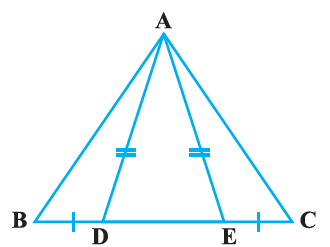
\includegraphics[width=1\columnwidth]{Figure1.png}

\label{fig}
\end{figure}

\section*{Solution}
1. Given points
A=$\myvec{
  7 \\
  6 \\
 }$
 and B=$\myvec{
  3 \\
  4 \\
 }$


\raggedright 2. If the point is lying on x-axis then y-axis will be zero i.e.. y=0

\fi
From the given information

\begin{align}
	\norm{\vec{x}-\vec{A}}^2 &=\norm{\vec{x}-\vec{B}}^2
	\\
	\implies
	\brak{\vec{x}-\vec{A}}^{\top} \brak{\vec{x}-\vec{A}} &= \brak{\vec{x}-\vec{B}}^{\top} \brak{\vec{x}-\vec{B}}
	\\
	\implies     \norm{\vec{x}}^2 - 2\vec{A}^{\top}\vec{x} + \norm{\vec{A}}^2 &= \norm{\vec{x}}^2 - 2\vec{B}^{\top}\vec{x} + \norm{\vec{B}}^2
	\\
	\text{or, }
	\brak{\vec{A}-\vec{B}}^{\top}   \vec{x}&= \frac{\norm{\vec{A}}^2 - \norm{\vec{B}}^2}{2}
		\label{eq:11/10/1/4}
\end{align}  
Since $\vec{x}$ lies on the $x$-axis,
\begin{align}
	\vec{x} &=k\vec{e}_1
\end{align}  
which, upon substituting in 
		\eqref{eq:11/10/1/4}
		yields
\begin{align}
	k = \frac{15}{2}
\end{align}
\iffalse
$\vec{(A-B)^{\top}x} = \frac{\|\vec{A}\|^2 - \|\vec{B}\|^2}{2}$\\ \vspace{2mm}
     $\myvec{0 & 1 \\ 4 & 2}x = $\myvec{0 \\ 30}\\ \vspace{2mm}
      $\myvec{0 & 1 & 0 \\ 4 & 2 & 30}$\\    \vspace{2mm}
      Divide by 2\\
      $\myvec{0 & 1 & 0 \\ 2 & 1 & 15}$\\    \vspace{2mm}
     $\myvec{2 & 1 & 15 \\ 0 & 1 & 0}
    \xleftarrow[]{R_2 \leftarrow R_1}$\\     \vspace{2mm}
    $\myvec{1 & \frac{1}{2} & \frac{15}{2} \\ 0 & 1 & 0}\xleftarrow[]{{R_1}=\frac{R_1}{2}}$\\            \vspace{2mm}
    $\myvec{1 & 0 & \frac{15}{2} \\ 0 & 1 & 0}\xleftarrow[]{{R_1}={R_1}-\frac{R_2}{2}}$\\             \vspace{2mm}
    $\myvec{1 & 0 & 7.5 \\ 0 & 1 & 0}$\\        \vspace{2mm}
on solving we get x = 7.5\\
\vspace{2mm}
  x=$\myvec{
  7.5 \\
  0 \\
 }$               			
\end{document}
\fi

\item 
%\label{chapters/11/10/1/4}
%\iffalse
\documentclass[journal,10pt,twocolumn]{article}
\usepackage{graphicx}
\usepackage[margin=0.5in]{geometry}
\usepackage[cmex10]{amsmath}
\usepackage{array}
\usepackage{booktabs}
\usepackage{makecell}
\title{\textbf{Line Assignment}}
\author{Hari Venkateswarlu}
\date{September 2022}
\usepackage[framemethod=tikz]{mdframed}
\newcommand{\myvec}[1]{\ensuremath{\myvec{#1}}}
\let\vec\mathbf
\newcommand{\mydet}[1]{\ensuremath{\begin{vmatrix}#1\end{vmatrix}}}
\providecommand{\mbf}{\mathbf}
\providecommand{\pr}[1]{\ensuremath{\Pr\left(#1\right)}}
\providecommand{\qfunc}[1]{\ensuremath{Q\left(#1\right)}}
\providecommand{\sbrak}[1]{\ensuremath{{}\left[#1\right]}}
\providecommand{\lsbrak}[1]{\ensuremath{{}\left[#1\right.}}
\providecommand{\rsbrak}[1]{\ensuremath{{}\left.#1\right]}}
\providecommand{\brak}[1]{\ensuremath{\left(#1\right)}}
\providecommand{\lbrak}[1]{\ensuremath{\left(#1\right.}}
\providecommand{\rbrak}[1]{\ensuremath{\left.#1\right)}}
\providecommand{\cbrak}[1]{\ensuremath{\left\{#1\right\}}}
\providecommand{\lcbrak}[1]{\ensuremath{\left\{#1\right.}}
\providecommand{\rcbrak}[1]{\ensuremath{\left.#1\right\}}}

\begin{document}

\maketitle
\paragraph{\textit{Problem Statement} - 
\fi
	\begin{figure}[!ht]
		\centering
 \includegraphics[width=\columnwidth]{chapters/11/10/1/4/figs/line.png}
		\caption{}
		\label{fig:11/10/1/4}
  	\end{figure}
	\\
	\solution 
\iffalse
 }
\begin{center}
    \label{tab:truthtable}
    \setlength{\arrayrulewidth}{0.2mm}
\setlength{\tabcolsep}{5pt}
\renewcommand{\arraystretch}{1.25}
    \begin{tabular}{|c|c|c|}
    \hline % <-- Alignments: 1st column left, 2nd middle and 3rd right, with vertical lines in between
      \large\textbf{Symbol} & \large\textbf{Co-ordinates} & \large\textbf{Description}\\
      \hline
       \large A & $\ \myvec{ 7\\ 6 }$ & co-ordinates of A \\
       \large B & $\ \myvec{ 3\\ 4 }$ & co-ordinates of B \\
	
	
      \hline
   \end{tabular}
 \end{center}\vspace{5mm}

\begin{figure}[h]
\centering
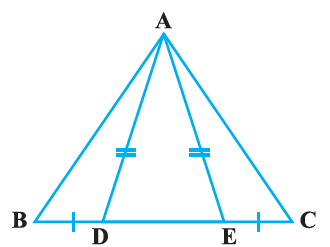
\includegraphics[width=1\columnwidth]{Figure1.png}

\label{fig}
\end{figure}

\section*{Solution}
1. Given points
A=$\myvec{
  7 \\
  6 \\
 }$
 and B=$\myvec{
  3 \\
  4 \\
 }$


\raggedright 2. If the point is lying on x-axis then y-axis will be zero i.e.. y=0

\fi
From the given information

\begin{align}
	\norm{\vec{x}-\vec{A}}^2 &=\norm{\vec{x}-\vec{B}}^2
	\\
	\implies
	\brak{\vec{x}-\vec{A}}^{\top} \brak{\vec{x}-\vec{A}} &= \brak{\vec{x}-\vec{B}}^{\top} \brak{\vec{x}-\vec{B}}
	\\
	\implies     \norm{\vec{x}}^2 - 2\vec{A}^{\top}\vec{x} + \norm{\vec{A}}^2 &= \norm{\vec{x}}^2 - 2\vec{B}^{\top}\vec{x} + \norm{\vec{B}}^2
	\\
	\text{or, }
	\brak{\vec{A}-\vec{B}}^{\top}   \vec{x}&= \frac{\norm{\vec{A}}^2 - \norm{\vec{B}}^2}{2}
		\label{eq:11/10/1/4}
\end{align}  
Since $\vec{x}$ lies on the $x$-axis,
\begin{align}
	\vec{x} &=k\vec{e}_1
\end{align}  
which, upon substituting in 
		\eqref{eq:11/10/1/4}
		yields
\begin{align}
	k = \frac{15}{2}
\end{align}
\iffalse
$\vec{(A-B)^{\top}x} = \frac{\|\vec{A}\|^2 - \|\vec{B}\|^2}{2}$\\ \vspace{2mm}
     $\myvec{0 & 1 \\ 4 & 2}x = $\myvec{0 \\ 30}\\ \vspace{2mm}
      $\myvec{0 & 1 & 0 \\ 4 & 2 & 30}$\\    \vspace{2mm}
      Divide by 2\\
      $\myvec{0 & 1 & 0 \\ 2 & 1 & 15}$\\    \vspace{2mm}
     $\myvec{2 & 1 & 15 \\ 0 & 1 & 0}
    \xleftarrow[]{R_2 \leftarrow R_1}$\\     \vspace{2mm}
    $\myvec{1 & \frac{1}{2} & \frac{15}{2} \\ 0 & 1 & 0}\xleftarrow[]{{R_1}=\frac{R_1}{2}}$\\            \vspace{2mm}
    $\myvec{1 & 0 & \frac{15}{2} \\ 0 & 1 & 0}\xleftarrow[]{{R_1}={R_1}-\frac{R_2}{2}}$\\             \vspace{2mm}
    $\myvec{1 & 0 & 7.5 \\ 0 & 1 & 0}$\\        \vspace{2mm}
on solving we get x = 7.5\\
\vspace{2mm}
  x=$\myvec{
  7.5 \\
  0 \\
 }$               			
\end{document}
\fi

\item 
\label{chapters/11/10/1/5}
\iffalse
\documentclass[journal,12pt,twocolumn]{IEEEtran}
\usepackage{graphicx}
\graphicspath{{./figs/}}{}
\usepackage{amsmath,amssymb,amsfonts,amsthm}
\newcommand{\myvec}[1]{\ensuremath{\begin{pmatrix}#1\end{pmatrix}}}

\let\vec\mathbf

\title{
Matrix-Lines
}
\author{Jyothsna Paluchuri-FWC22059\\}
\begin{document}
\maketitle
\tableofcontents
\bigskip
\section{Problem Statement}
\fi
	\begin{figure}[!ht]
		\centering
 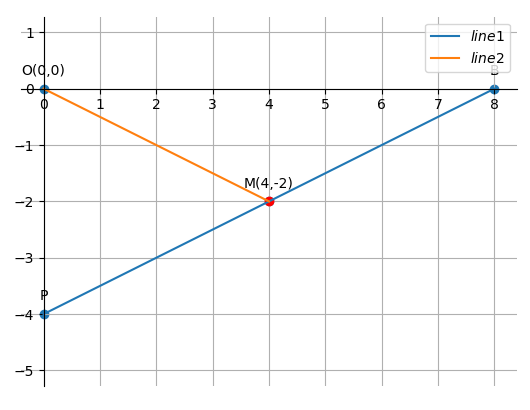
\includegraphics[width=\columnwidth]{chapters/11/10/1/5/figs/line.png}
		\caption{}
		\label{fig:11/10/1/5}
  	\end{figure}
	\\
	\solution
\iffalse
\section{Construction}
\begin{figure}[h]
    \centering
\includegraphics[width=\columnwidth]{line.png}
    \caption{Equation of the slope}
    \label{fig:my_label}
\end{figure}
\vspace{2cm}
\begin{table}[h]
    \centering
    \begin{tabular}{|c|c|c|c|}
       \hline
       \textbf{Symbol}&\textbf{Value}&\textbf{Description}  \\
       \hline
	    $\vec{P}$ & $\myvec{
		    0\\
		    -4}$
	    & Point on Y-axis\\
        \hline
	    $\vec{B}$ & $\myvec{8\\0}$
 & Point on X-axis\\
        \hline
	    $\vec{0}$ & $\myvec{0\\0}$
 & Origin\\
        \hline
    \end{tabular}
    \caption{Parameters}
    \label{tab:my_label}
\end{table}


\section{Solution}
Given that resultant line passes through origin and mid point of the line segment joining point P(0,-4) and B(8,0) \\
\\
\\
given ${\vec{P}}$=$\myvec{
  0\\
  -4}$
 , ${\vec{B}}$=$\myvec{
  8\\
  0}$
  
 \fi 
The mid point of $PB$ is
\begin{align}
\vec{M} &=\frac{1}{2}(\vec{P}+\vec{B})
	= \myvec{4 \\ -2}  
\end{align}
The direction vector of line joining $\vec{O}, \vec{M}$ is 
\begin{align}
\vec{m}&=\vec{O}-\vec{M}
 = -\vec{M}
\end{align}
which can be expressed as
\begin{align}
	\myvec{1 \\ -\frac{1}{2}}
\end{align}
Thus the slope is
\begin{align}
	m = -\frac{1}{2}
\end{align}
\iffalse
\textbf{The direction vector of a line expressed as}
\begin{align}
\implies\vec{m} &= \begin{pmatrix}1 \\ m \\ \end{pmatrix}
\end{align}

\textbf{By solving equation (5) and (6),we get the slope of $\vec{O}$ $\vec{M}$ line}
\begin{align}
        \boxed{m=-0.5}
 \end{align}

\section{Software}
Download the following code using,
\begin{table}[h]
    \centering
    \begin{tabular}{|c|}
    \hline \\
   https://github.com/jyothsna777/jyothsna-fwc.git  \\
         \\
\hline
    \end{tabular}
\end{table}
\\
and execute the code by using command
\begin{center}
\textbf{Python3 lines.py}\\
\end{center}

\section{Conclusion}
Hence the slope of line $\vec{O}$ $\vec{M}$ lineis $\vec{m}$=-0.5

\end{document}
\fi

\item 
\label{chapters/11/10/1/6}
\iffalse
\documentclass[journal,12pt,twocolumn]{IEEEtran}
\usepackage[none]{hyphenat}
\usepackage{graphicx}
\usepackage{listings}
\usepackage[english]{babel}
\usepackage{graphicx}
\usepackage{caption} 
\usepackage{amsmath}
\usepackage{hyperref}
\usepackage{booktabs}
\usepackage{array}


\title{\textbf{\\Assignment on line}}
\author{Sireesha Abbavaram - FWC22060}
\begin{document}
\maketitle


\section{Question}
\textbf{\textit{Class 11, Exercise 10.1, Q(6):}
\fi
	\begin{figure}[!ht]
		\centering
 \includegraphics[width=\columnwidth]{chapters/11/10/1/6/figs/triangle.png}
		\caption{}
		\label{fig:11/10/1/6}
  	\end{figure}
\iffalse
}

\begin{figure}[h!]
\centering
\includegraphics[scale=0.35]{triangle.png}
\centering
\caption{Traingle ABC}
\end{figure}


\section{Solution}
\raggedright 
\vspace{0.25cm}
Let A,B and C be the vertices of a given traingle with coordinates $\myvec{
4 \\
4
}
, \myvec{
3 \\
5
}
 and \myvec{
-1 \\
-1
} $
\raggedright
. we have verify whther the given vertices are of right angled triangle or not.\\
\begin{center}
\raggedright
Let The directional vector of two vectors A and B is given as AB (m1)=A-B.
\end{center}
\vspace{0.25cm}
\begin{center}
The directional vector of the vectors B and C is given as BC (m2)=B-C.
\end{center}
\vspace{0.25cm}
\begin{center}
The directinal vector of the vectors C and A is given as CA (m3)=C-A.
\end{center}
\vspace{0.25cm}
The angle between any two vectors is given by
\boldmath
\\ $ cos b =\frac{(m1)^T(m2)}{||m1|| ||m2||}  equation-1$
\unboldmath
\vspace{0.5cm}\raggedright\\
Where b is the angle between the two vectors .
when the angle b=90 ,we get cos 90=0.
\vspace{0.5cm}\raggedright\\
It implies that the numerator of the equation 1 should be zero.

\vspace{0.25cm}
 In order to prove that the triangle is right angled we have to show any two vectors should be orthogonal to each other.
 
\vspace{0.25cm}\raggedright
So we need to show $(A-B)^T(B-C) or (B-C)^T(C-A) or (C-A)^T(A-B) $ is equal to zero.
\fi

\vspace{0.5cm}\raggedright
\begin{align}
	\vec{C}-\vec{A}&=\myvec{
-5 \\
	-5},
\\
	\vec{A}-\vec{B}&=\myvec{
1 \\
-1 
}
\\
	\implies \brak{\vec{C}-\vec{A}}^{\top}
	\brak{\vec{A}-\vec{B}}&=0
\end{align}
Thus, $AB \perp AC$.
\iffalse
\vspace{0.25cm}\raggedright
Thus we have right angle at the vertex A.


\vspace{0.2cm}
\section*{Construction}
\centering
\vspace{0.2cm}
{
\setlength\extrarowheight{2pt}
\begin{tabular}{|c|c|c|}
	\hline
	\textbf{Symbol}&\textbf{Value}&\textbf{Description}\\
	\hline
	A & (4,4) & Vertex A\\
	\hline
	B & (3,5) & Vertex B\\
	\hline
	C & (-1,-1) & Vertex C\\
	\hline
	
\end{tabular}
}

\vspace{0.6cm}
Get the python code of the figures from
\begin{table}[h]
\large
\centering
\begin{tabular}{|l|}
\hline
https://github.com/Sireesha1602/sireesha/
\\blob/main/line assignment \\
\hline
\end{tabular}

\end{table}




\end{document}
\fi

\item 
\label{chapters/11/10/1/8}
\iffalse
\documentclass[10pt, a4paper]{article}
\usepackage[a4paper,outer=1.5cm,inner=1.5cm,top=1.75cm,bottom=1.5cm]{geometry}

\twocolumn
\usepackage{graphicx}

\usepackage{hyperref}
\usepackage[utf8]{inputenc}
\usepackage{amsmath}
\usepackage{physics}
\usepackage{amssymb}
\begin{document}
\title{Assignment-4}
\author{Name:C.CHANDANA\and Email :  \url{cheenepallichandana531@gmail.com}}
%\{ Wireless Communication (FWC)}
\date{30-sep-2022}
\maketitle



\section{Problem}
\fi
If three points $(x, -1), (2, 1)$ and $(4, 5)$ are collinear, find the value of $x$.
\\
\solution 
	\begin{figure}[!ht]
		\centering
 \includegraphics[width=\columnwidth]{chapters/11/10/1/8/figs/sline.png}
		\caption{}
		\label{fig:11/10/1/8}
  	\end{figure}
	\iffalse
\begin{center}
	\fi
	Let
\begin{align} \label{eq:11/10/1/8}
	\vec{A}=\myvec{ x\\ -1 },
	\vec{B}=\myvec{ 2\\ 1 },
\vec{C}=\myvec{ 4\\ 5 }.
\end{align}
Then
\begin{align}
\vec{A}-\vec{B}
	&=\myvec{ x-2\\ -2 }
	\\
\vec{A}-\vec{C}
	&=\myvec{ 4-x\\ 6 }
\end{align}
Forming the collinearity matrix
using 
	\eqref{eq:normal_line-collinear},
\begin{align} 
\myvec{ x-2 & -2\\ 4-x & 6  } 
	\xleftrightarrow[]{{R_1=3R_1+R-2}}
=\myvec{
2x-2 &0 \\ 
 4-x& 6
}
\end{align}

\iffalse

In the problem they have given that three points lie on a line, thats means these three points are collinear.\\

If  points on a line  are  collinear, rank of matrix is " 1 "then the vectors are in linearlydependent.\\
For 2 × 2 matrix Rank =1 means Determinant is 0.\\

Through pivoting,we obtain\\
\begin{align}
=\myvec{ x-2 & -2\\ 4-x & 6 \ } \\ 
\end{align}
\begin{align}
=\myvec{
x-2 &-2 \\ 
 4-x& 6
}\overset{R1=3R1+R2}{\rightarrow}
=\myvec{
2x-2 &0 \\ 
 4-x& 6
}
\end{align} 
\fi
	If the rank of the matrix is 1, any one of the rows must be zero. So, making the first element in the above matrix 0,
\begin{align}
x=1
\end{align} 

\iffalse

\begin{align}\label{eq:11/10/1/8}
x=1 \\
\end{align} 

Hence proved.\\
\section{Construction}
 \begin{figure}[h]
\centering
\includegraphics[scale=0.4]{sline.png} 
\caption{}
\end{figure}
\section{Code}
*Verify the above proofs in the following code.\\
\framebox{
\url{https://github.com/chandana531/FWC/tree/main/matrix/line}}	
\bibliographystyle{ieeetr}
\end{document}
\fi

\item 
\label{chapters/11/10/1/9}
\iffalse
\documentclass[journal,12pt,twocolumn]{IEEEtran}
\usepackage[none]{hyphenat}
\usepackage{graphicx}
\usepackage{listings}
\usepackage[english]{babel}
\usepackage{graphicx}
\usepackage{caption} 
\usepackage{amsmath}
\usepackage{hyperref}
\usepackage{booktabs}
\usepackage{array}
\usepackage{stix}


\title{\textbf{\\Line Assignment}}
\author{kanekal kousar}
\date{September 2022}

\providecommand{\norm}[1]{\left\lVert#1\right\rVert}
\providecommand{\abs}[1]{\left\vert#1\right\vert}
\let\vec\mathbf
\newcommand{\myvec}[1]{\ensuremath{\myvec{#1}}}
\newcommand{\mydet}[1]{\ensuremath{\begin{vmatrix}#1\end{vmatrix}}}
\providecommand{\brak}[1]{\ensuremath{\left(#1\right)}}

\begin{document}
\maketitle


\section{Question}
\textbf{\textit{Class 11, Exercise 10.1, Q(9):} 
\fi
Without using distance formula, show that points (– 2, – 1), (4, 0), (3, 3) and (–3, 2) are the vertices of a parallelogram.
	\begin{figure}[!ht]
		\centering
 \includegraphics[width=\columnwidth]{chapters/11/10/1/9/figs/paralellogram.png}
		\caption{}
		\label{fig:11/10/1/9}
  	\end{figure}
	\\
	\solution See Fig. 
		\ref{fig:11/10/1/9}.
\iffalse
}

\section{Solution}
\raggedright 

\begin{figure}[h!]
\centering
\includegraphics[scale=0.5]{fig/paralellogram.png}  
\caption{paralellogram ABCD}
\end{figure}

\vspace{0.25cm}
We can prove that the points are the vertices of a parallelogram if the direction vectors of opposite lines are equal

Consider  figure I,where
\fi


\begin{align}
\vec{A}=\myvec{-2 \\ -1  },  \vec{B}=\myvec{ 4\\ 0 }, 
\vec{C}=\myvec{3 \\ 3  },  \vec{D}=\myvec{-3 \\ 2  }
\end{align}
and
\begin{align}
	\vec{P} &=\vec{B}-\vec{A}=\myvec{6 \\ 1 \\ }
	\\
	\vec{Q}&=\vec{C}-\vec{D}=\myvec{6 \\ 1 \\ }
	\\
	\vec{R}&=\vec{A}-\vec{C}=\myvec{1 \\ -3 \\ }
	\\
	\vec{S}&=\vec{A}-\vec{D}=\myvec{1 \\ -3 \\ }
\end{align}
Since
$\vec{P}=\vec{Q}$
and 
$\vec{R}=\vec{S}$, from  
	  \eqref{eq:two-pgm},
$ABCD$ is a 
parallelogram
\iffalse

\section*{Construction}
\centering
\vspace{0.2cm}
{
\setlength\extrarowheight{2pt}
\begin{tabular}{|c|c|c|}
	\hline
	\textbf{Symbol}&\textbf{Value}&\textbf{Description}\\
	\hline
	A & $\myvec{-2 \\ -1 \\ }$ & Vertex A\\
	\hline
	B & $\myvec{4 \\ 0 \\ }$ & Vertex B\\
	\hline
	C &$\myvec{3 \\ 3 \\ }$ & Vertex C\\
	\hline
	D & $\myvec{-3 \\ 2 \\ }$ & Vertex D\\
	\hline
	P &$\myvec{1 \\ 6 \\ }$&vector AB\\
	\hline
	Q&$\myvec{1 \\ 6 \\ }$&vector DC\\
	\hline
	R&$\myvec{1 \\ -3 \\ }$&vector BC\\
	\hline
	S&$\myvec{1 \\ -3 \\ }$&vector AD\\
	\hline
\end{tabular}
}

\vspace{0.6cm}
Get the python code of the figures from
\begin{table}[h]
\large
\centering
\framebox{
\url{https://github.com/kkousar/KOUSAR_FWC/blob/main/line_assignment/code/line.py}}
\bibliographystyle{ieeetr}

\end{table}



\end{document}
\fi

\item 
\label{chapters/11/10/1/10}
\iffalse
\def\mytitle{PYTHON PROGRAMMING ON MATRICES}
\def\myauthor{Revathi pamujula}
\def\contact{revathipamujula111@gmail.com}
\def\mymodule{Future Wireless Communication (FWC)}


\documentclass[10pt, a4paper]{article}
\usepackage[a4paper,outer=1.5cm,inner=1.5cm,top=1.75cm,bottom=1.5cm]{geometry}

\twocolumn
\usepackage{graphicx}
%\usepackage{karnaugh-map}
\usepackage{tabularx}
\usepackage{hyperref}
\usepackage[utf8]{inputenc}
\usepackage{amsmath}
%\usepackage{physics}
\usepackage{amssymb}
\usepackage{watermark}
\renewcommand*\familydefault{\sfdefault}
\usepackage{lipsum}
\usepackage{xcolor}
\usepackage{listings}
\let\vec\mathbf
\lstset{
frame=single, 
breaklines=true,
columns=fullflexible
}

\begin{document}
\title{\mytitle}
\author{\myauthor\hspace{1em}\\\contact\\FWC22045\hspace{6.5em}IITH\hspace{0.5em}\mymodule\hspace{6em}Matrix:Lines}

%\{ Wireless Communication (FWC)}
\date{}
\maketitle


  \section{Problem}
  \fi
\\
\solution See Fig. 
		\ref{fig:11/10/1/10}.
	\begin{figure}[!ht]
		\centering
 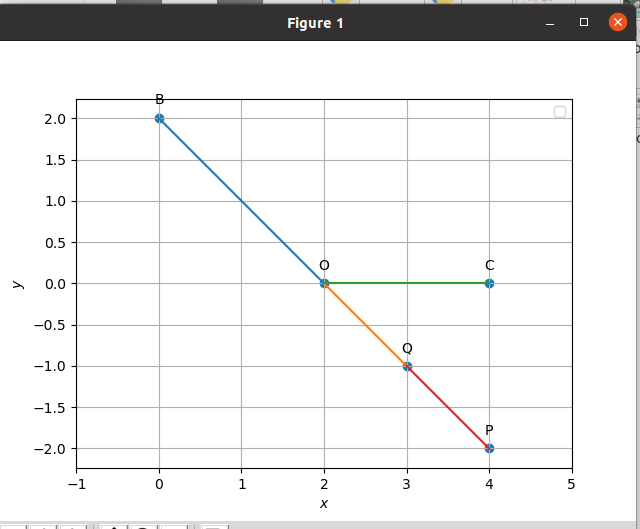
\includegraphics[width=\columnwidth]{chapters/11/10/1/10/figs/fig.png}
		\caption{}
		\label{fig:11/10/1/10}
  	\end{figure}

	\iffalse
\section{Solution}
\textbf{Given that:}
\begin{center}

%\boldmath
	\fi
	Let 
\begin{align}
\vec{P}=\myvec{ 3\\ -1 },
\vec{Q}=\myvec{ 4\\ -2 }
\end{align}
Then 
\begin{align}
	\vec{C}=\vec{P}-\vec{Q}
=\myvec{ -1\\ 1 }
\end{align}
The desired angle is given by
\begin{align}
	\cos\theta&=\frac{\vec{C}^{T}\vec{e}_1}{\norm{\vec{C}}\norm{\vec{e}_1}}
	\\
	&= -\frac{1}{\sqrt{2}}
	\\
	\implies 
	\theta&=135\degree
 \end{align}
 \iffalse
\begin{figure}[h!]
  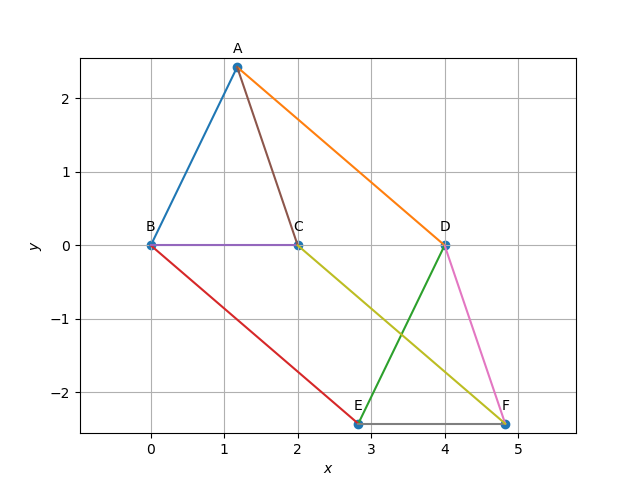
\includegraphics[scale=0.5]{fig.png}
  \caption{line assignment }
  \label{fig:line assignment}
\end{figure}
\end{document}
\fi

\item 
\label{chapters/11/10/1/11}
\iffalse
\documentclass[10pt,a4paper]{report}
%\usepackage[latin1]{inputenc}
\usepackage[utf8]{inputenc}
\usepackage{amsmath}
\usepackage{amsfonts}
\usepackage{amssymb}
\usepackage{graphicx}
\usepackage{multicol}
\usepackage{tabularx}
\usepackage{tikz}
\usetikzlibrary{arrows,shapes,automata,petri,positioning,calc}
\usepackage{hyperref}
\usepackage{tikz}
\usetikzlibrary{matrix,calc}
\usepackage[margin=0.5in]{geometry}
% ---- power functions -----% 
\newcommand{\myvec}[1]{\ensuremath{\begin{pmatrix}#1\end{pmatrix}}}
\let\vec\mathbf

\providecommand{\norm}[1]{\left\lVert#1\right\rVert}
\providecommand{\abs}[1]{\left\vert#1\right\vert}
\let\vec\mathbf

\newcommand{\mydet}[1]{\ensuremath{\begin{vmatrix}#1\end{vmatrix}}}
\providecommand{\brak}[1]{\ensuremath{\left(#1\right)}}
\providecommand{\lbrak}[1]{\ensuremath{\left(#1\right.}}
\providecommand{\rbrak}[1]{\ensuremath{\left.#1\right)}}
\providecommand{\sbrak}[1]{\ensuremath{{}\left[#1\right]}}
%-------end power functions----%
\newenvironment{Figure}
  {\par\medskip\noindent\minipage{\linewidth}}
  {\endminipage\par\medskip}
\begin{document}
%--------------------logo figure-------------------------%
\begin{figure*}[!tbp]
  \centering
  \begin{minipage}[b]{0.4\textwidth}
    
\includegraphics[scale = 0.05]{iitlogo.jpg}
  \end{minipage}
  \hfill
  \vspace{5mm}\begin{minipage}[b]{0.4\textwidth}
\raggedleft  
\includegraphics[scale = 0.10]{nrc.png}\

  \end{minipage}\vspace{0.2cm}
\end{figure*}
%--------------------name & rollno-----------------------
\raggedright \textbf{Name}:\hspace{1mm} D. Siva Krishna\hspace{3cm} \Large \textbf{Assignment-4}\hspace{2.5cm} % 
\normalsize \textbf{Roll No.} :\hspace{1mm} FWC22065\vspace{1cm}
\begin{multicols}{2}

%----------------problem statement--------------%
\raggedright \textbf{Problem Statement:}\vspace{2mm}
\raggedright \\
\fi
	The slope of a line is double of the slope of another line. If tangent of the angle between them is 1/3, find the slopes of the lines.
	\begin{figure}[!ht]
		\centering
 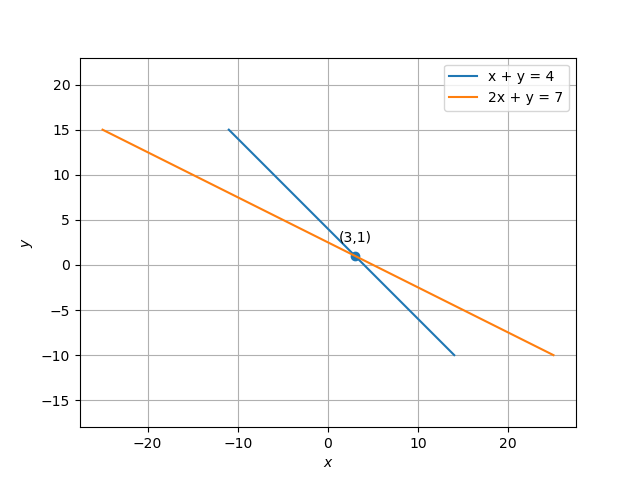
\includegraphics[width=\columnwidth]{chapters/11/10/1/11/figs/line.png}
		\caption{}
		\label{fig:11/10/1/11}
  	\end{figure}
	\iffalse
\vspace{5mm}
%-----------------------------solution---------------------------
\raggedright \textbf{SOLUTION}:\vspace{2mm}\\

%---------given----------------%
\raggedright \textbf{Given}:\vspace{2mm}\\
Slope of one line is double of the slope of the other line. \\\vspace{1mm}
\fi
\\
\solution 
The direction vector of a line is expressed as
\begin{align}
\vec{m}=\myvec{1\\m}
\end{align}
where  $m$ is defined to be the slope of the line. If the angle between the lines be $\theta$,
\begin{align}
\tan \theta = \frac{1}{3}
\implies \cos \theta=\frac{3}{\sqrt{10}}
\end{align}
\iffalse
%--------------steps----------------------%
\textbf{Input Parameters:}
\vspace{2mm}


\begin{tabular}{|c|c|c|}
	\hline
	\textbf{Symbol}&\textbf{Value}&\textbf{Description}\\
	\hline
	$\vec{m_1}$ &\myvec{1\\m}& Direction vector\\
	\hline
    $\vec{m_2}$ &\myvec{1\\2m}&Direction vector\\
	\hline
    $\tan\theta$ &1/3& Angle\\
	\hline
\end{tabular}
\\
\vspace{10cm}
\fi
The angle between two vectors is then expressed as
\iffalse
\begin{align}
\cos \theta = \frac{^\top \textbf{B}}{\norm{\textbf{A}}\norm{\textbf{B}}}
\end{align} 
%Substituting the \vec{m_1} and \vec{m_2} in the above equation
\\
\fi
\begin{align}
	\frac{3}{\sqrt{10}} &= \frac{\vec{m}_1^\top \vec{m}_2}{\norm{\vec{m}_1}\norm{\vec{m}_2}}
	\\
	&= \frac{\myvec{1 &  m}\myvec{1 \\ 2m}}{\norm{\myvec{1\\m}}\norm{\myvec{1\\2m}}}
\\
	&= \frac{2m^2 +1}{\sqrt{m^2 + 1}\sqrt{4m^2 + 1}}
	\\
	\implies \frac{9}{10}&=\frac{4m^4 + 4m^2 +1}{4m^4 + 5m^2 +1}
\\
	\text{or, } 4m^4 - 5m^2 +1 = 0
\end{align}
\iffalse
Let $m^2$ = x and substituting it in above equation we get a quadratic equation.
\begin{align}
	4x^2 -5x +1 = 0
\end{align}
From the formula of fining roots of a quadratic equation
\begin{align}
	\frac{-b\pm \sqrt{b^2 - 4ac}}{2a}
	\\
	\\
	\frac{5\pm \sqrt{\left (-5\right )^2 - 16}}{8}
	\\
	x= 1 (or) x = 1/4
\end{align}
\\
The slope of the first line is
\\
\fi
yielding
\begin{align}
m=\pm \frac{1}{2}, 
\pm 1
\end{align}
\iffalse
$\therefore $ Slope of second line is
\begin{center}
$ 2m=\pm 1$\\
    (or)\\
    $2m=\pm 2$
\end{center}
\begin{center}
 \includegraphics[width=0.5\textwidth]{line.png}  
 \end{center}\vspace{1mm}
\raggedright  Download the code \\
Github link:{Assignment-4}.
\end{multicols}
\end{document}
\fi

\item 
\label{chapters/11/10/1/12}
\iffalse 
\documentclass[journal,12pt,twocolumn]{IEEEtran}
\usepackage{graphicx}
\graphicspath{{./figs/}}{}
\usepackage{amsmath,amssymb,amsfonts,amsthm}
\newcommand{\myvec}[1]{\ensuremath{\begin{pmatrix}#1\end{pmatrix}}}

\let\vec\mathbf

\title{
Matrix-Lines
}
\author{R.Radhika}
\begin{document}
\maketitle
\tableofcontents
\bigskip
\section{Problem Statement}
\fi
\\
\solution 
	\begin{figure}[!ht]
		\centering
 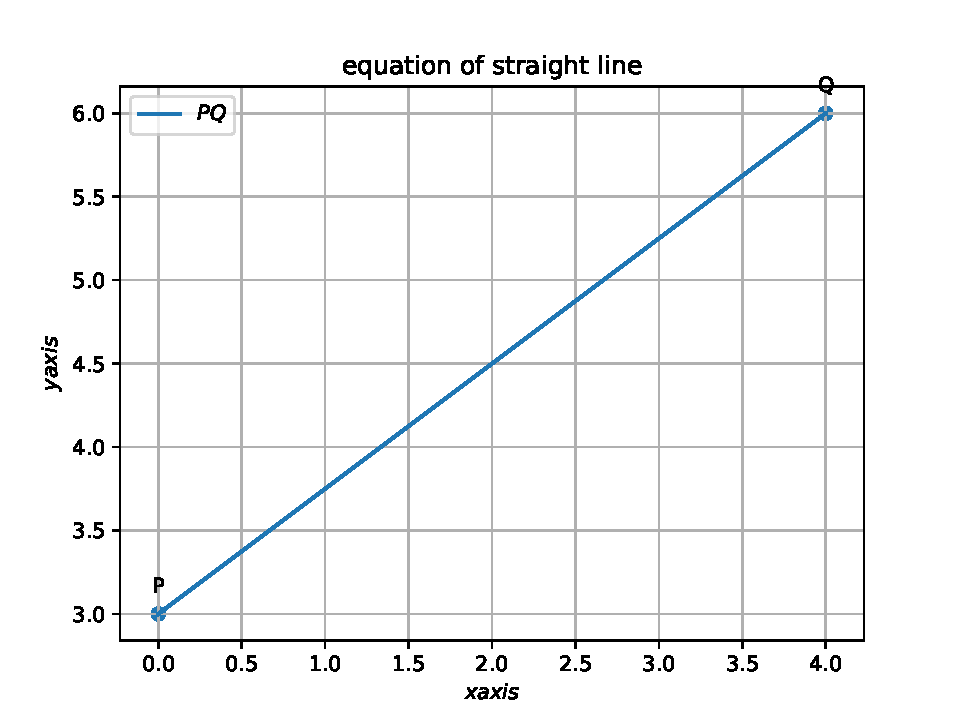
\includegraphics[width=\columnwidth]{chapters/11/10/1/12/figs/figure.pdf}
		\caption{}
		\label{fig:11/10/1/12}
  	\end{figure}
\iffalse
\section{Construction}
\begin{figure}[h]
    \centering
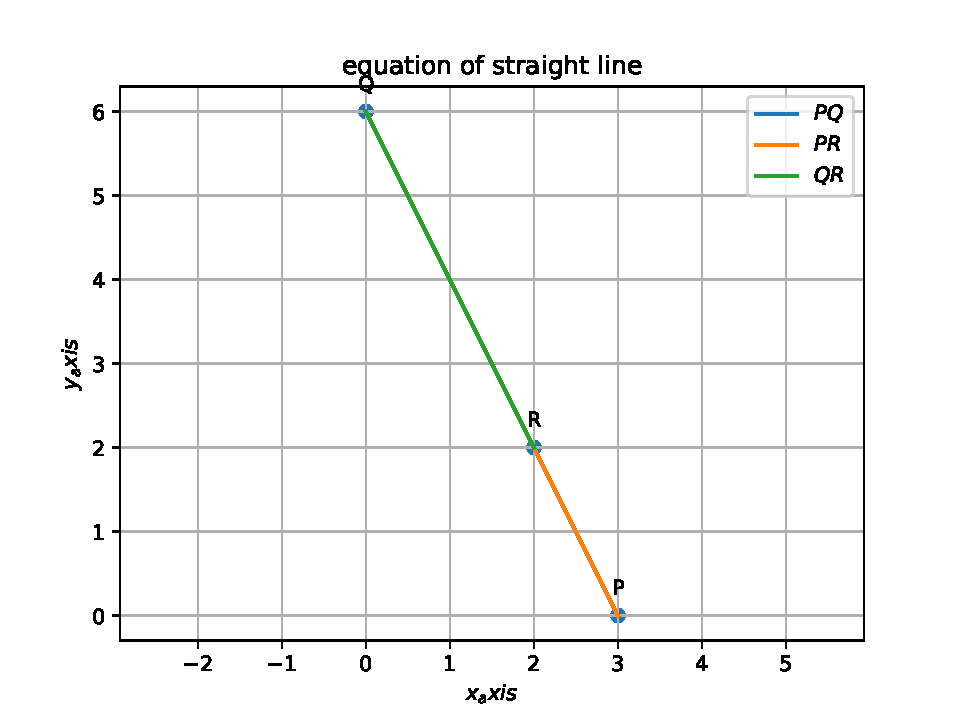
\includegraphics[width=\columnwidth]{figure.pdf}
    \caption{Equation of the slope}
    \label{fig:my_label}
\end{figure}
\vspace{2cm}
\begin{table}[h]
    \centering
    \begin{tabular}{|c|c|c|}
       \hline
       \textbf{Symbol}&\textbf{Value}&\textbf{Description}  \\
       \hline
	    $\vec{A}$ & $\myvec{
		    x_1\\
		    y_1}$
	    & Point on X-axis\\
        \hline
	    $\vec{B}$ & $\myvec{h\\k}$
 & Point on Y-axis\\
        \hline
        \hline
        A & k-y1=m(h-x1) & Given Condition\\
        \hline
    \end{tabular}
    \caption{Parameters}
    \label{tab:my_label}
\end{table}


\section{Solution}
Given that resultant line passes through point(x1,y1) and (h,k) (let prove the equation in vector form by line eqation ) \\
\\
\\
\fi
Given 
\begin{align}
\vec{A}=\myvec{
  x_1\\
  y_1}
 , \vec{B}=\myvec{
  h\\
  k}
\end{align}

\iffalse
\textbf{First Method}:\\
condition is	
\begin{equation}
	{\vec{n^{\top}}\vec{{m}}} = 0 \\     \label{eq-1}
\end{equation}	
m is 
\fi
The direction vector
\begin{align}
	\vec{m} &= \vec{B}-\vec{A}
	\\
	&=
	\myvec{
  h-x_1\\
  k-y_1
  }
   \equiv
	\myvec{
1\\
	\frac{ k-y_1}{h-x_1}
  }
\end{align}
which yields the desired relation from 
		\eqref{eq:two-dir-vec}.
\iffalse
\begin{equation}
 			\myvec{
					-m& 1}\myvec{
  h-x_1\\
  k-y_1
  }
   = 0  \label{eq-4}
\end{equation}
by solving eq-4
\begin{equation}
	\myvec{
 -m (h-x_1))+(k-y_1}=0
\end{equation}
Then the equation becomes\\

$\myvec{
  k-y_1)=m(h-x_1}$\\
Therefore the Resultant Equation of line is\\
\begin{equation}
	\myvec{
  k-y_1)=m(h-x_1}
\end{equation}
\begin{table}[h]
    \centering
    \begin{tabular}{|c|}
    \hline \\
           \myvec{
  k-y_1)=m(h-x_1}\\
         \\
\hline
    \end{tabular}
\end{table}\\
\textbf{Second Method}:\\
given ${\vec{A}}$=$\myvec{
  x_1\\
  y_1}$
  ${\vec{B}}$=$\myvec{
  h\\
  k}$\\
C=$\myvec{
  \frac{x_1+h}{2}\\
  \frac{y_1+k}{2}
}$\\
m is the direction vector\\

		 m=C-A\\
		 
		 m=B-C\\
		 		 
m=$\myvec{
  \frac{x_1+h}{2}-x_1\\
  \frac{y_1+k}{2}-y_1
}$\\

 m=2$\myvec{
  \frac{h-x_1}{2}\\
  \frac{k-y_1}{2}
}$\\

m=$\myvec{
  {h-x_1}\\
  {k-y_1}
}$\\

condition is	
\begin{equation}
	{\vec{n^{\top}}\vec{{m}}} = 0 \\     \label{eq-1}
\end{equation}
\begin{equation}
 			\myvec{
					-m& 1}\myvec{
  h-x_1\\
  k-y_1
  }
   = 0  \label{eq-4}
\end{equation}
by solving eq-4
\begin{equation}
	\myvec{
 -m (h-x_1))+(k-y_1}=0
\end{equation}
Then the equation becomes\\

$\myvec{
  k-y_1)=m(h-x_1}$\\
Therefore the Resultant Equation of line is\\
\begin{equation}
	\myvec{
  k-y_1)=m(h-x_1}
\end{equation}			 


\textbf{Third Method}:\\
\begin{equation}
	{\vec{n^{\top}}\vec{{m}}} = 0 \\     \label{eq-1}
\end{equation}		
\begin{equation}
	{\vec{n^{\top}}\vec{({x}-A)}} = 0 \\     \label{eq-2}
\end{equation}
\begin{equation}
	{\vec{n^{\top}}\vec{({x}-B)}} = 0      \label{eq-3}
\end{equation}


 The Equation of line through ${\vec{A}}$  from 1 is\\
\begin{equation}
	\vec{n^{\top}}\myvec{ 
	\myvec{
  x\\
  y}
  - \label{eq-4}
	\myvec{
  x_1\\
  y_1}}
   = 0 \
\end{equation}
\\
Equation of line passing through ${\vec{B}}$ from 2 is\\
\begin{equation}
	\vec{n^{\top}}\myvec{ 
	\myvec{
  x\\
  y}
  - \label{eq-5}
	\myvec{
  h\\
  k}}
  = 0 \
\end{equation}
\\
Now by solving eq3,\\
\begin{equation}
	\vec{n^{\top}}
	\myvec{
  x-x_1\\
  y-y_1
}
  = 0 \label{eq-6}
\end{equation}
 
Now by solving eq4,\\
\begin{equation}
	\vec{n^{\top}}
	\myvec{
  x-h\\
  y-k
}
  = 0 \label{eq-7}
\end{equation}
 \\
 From eq5 and eq6 we can prove the equation ${\vec{n}}$,\\
 \\
 \begin{equation}
 			\myvec{
					-m& 1}\myvec{
  x-x_1& y-y_1\\
  x-h & y-k
 }
	 = 0   \
\end{equation}\\
 by solving 7 th equation\\
 \begin{equation}
	\myvec{
  k-y_1)=m(h-x_1}
\end{equation}
\\
Therefore the Resultant Equation of line is ${\vec{n^{\top}}\vec{X}} = c$ 
\\
 \begin{equation}
	\myvec{
  k-y_1)=m(h-x_1}
\end{equation}

\section{Software}
Download the following code using,
\begin{table}[h]
    \centering
    \begin{tabular}{|c|}
    \hline \\
         https://github.com/Radhikarkv/fwcproject.git  \\
         \\
\hline
    \end{tabular}
\end{table}
\\
and execute the code by using command
\begin{center}
\textbf{Python3 lineassign.py}\\
\end{center}

\section{Conclusion}
prove the equation of a line passes trough a points$(x_1,y_1)$,(h,k) if slope of the line is m i.e $(k-y_1)=m(h-x_1)$.

\end{document}
\fi

\item 
\label{chapters/11/10/1/13}
\iffalse
\documentclass[10pt, a4paper]{article}
\usepackage[a4paper,outer=1.5cm,inner=1.5cm,top=1.75cm,bottom=1.5cm]{geometry}

\twocolumn
\usepackage{graphicx}

\usepackage{hyperref}
\usepackage[utf8]{inputenc}
\usepackage{amsmath}
\usepackage{physics}
\usepackage{amssymb}
\begin{document}
\title{Assignment-4}
\author{Name:A.SUSI\and Email :  \url{susireddy9121@gmail.com}}
%\{ Wireless Communication (FWC)}
\date{30-sep-2022}
\maketitle



\section{Problem}
\fi
\solution 
\iffalse
\section{Solution}
\begin{center}
The input given 
\boldmath
\fi 
Let
\begin{align} 
\vec{A}=\myvec{ h\\ 0 },
\vec{B}=\myvec{ a\\ b },
\vec{C}=\myvec{ 0\\ k }
\end{align}
Forming the matrix in 
	\eqref{eq:normal_line-collinear}, we obtain, upon row reduction
	\iffalse
\begin{align}
\myvec{ h-a & -b\\ h & -k  } 
\end{align}
Using row reduction, 


In the problem they have given that three points lie on a line, thats means these three points are collinear.\\
If  points on a line  are  collinear, rank of matrix is "1"then the vectors are in linearlydependent.\\
For 2 × 2 matrix Rank =1 means Determinant is 0.\\
Through pivoting,we obtain\\
\fi
\begin{align}\label{eq:}
\myvec{ h-a & -b\\ h & -k  }  
	\xleftrightarrow[]{{\frac{R_1}{h-a}}}\myvec{
1 &\frac{-b}{h-a} \\ 
 h& -k
}
	\\
	\xleftrightarrow[]{R_2\rightarrow R_2-hR_1}
\myvec{
1 &\frac{-b}{h-a} \\ 
 0&-k+\frac{bh}{h-a} 
}
\end{align} 
For obtaining a rank 1 matrix, 
\iffalse

if the rank of the matrix is 1 means any one of the row must be zero.So, making the last element in the matrix to 0.\\
\fi
\begin{align}
	-k+\frac{bh}{h-a}&=0
	\\
	\implies \frac{a}{h}+\frac{b}{k}&=1 
\end{align} 
upon simplification.
\iffalse

Hence proved.\\
\section{Construction}
 \begin{figure}[h]
\centering
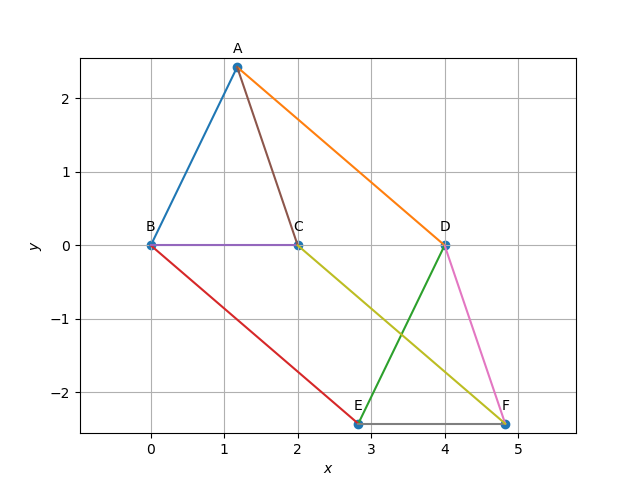
\includegraphics[scale=0.4]{fig.png} 
\caption{}
\end{figure}
\section{Code}
*Verify the above proofs in the following code.\\
\framebox{
\url{https://github.com/Susi9121/FWC/tree/main/matrix/line}}	
\bibliographystyle{ieeetr}
\end{document}
\fi


\end{enumerate}
